\documentclass{beamer}
\usepackage{graphicx}
\usepackage{amsmath}
\usepackage{textcomp}
\usepackage{tikz}

\usetikzlibrary{positioning}

\usetheme{Antibes}
\usecolortheme{beaver}

\title{Cluedo}
\author{Laura van de Braak, Luuk Boulogne \& Ren\'e Mellema}
\date{\today}


\begin{document}

\begin{frame}
    \titlepage
\end{frame}

\begin{frame}{Content}
  \tableofcontents
\end{frame}

\section{Introduction}

\begin{frame}{Rules of Cluedo}
  
\end{frame}

\section{Theory}
\begin{frame}{Theory}

\end{frame}

\subsection{Model}
\begin{frame}{Model}
    \begin{itemize}
        \item Normal Kripke model
        \item One state for each possible dealing of cards
        \item States are natural numbers
        \item Valuation is a dealing
        \item Relation if agent cannot differentiate
    \end{itemize}
\end{frame}

\begin{frame}{Model}
    \begin{itemize}
        \item Automatically encodes game rules
        \item All knowledge updates are as intended
        \item Total number of states:
            \begin{itemize}
                \item Simplified: $60.480$
                    \pause
                \item Full: $44.460.928.512.000$
            \end{itemize}
    \end{itemize}
\end{frame}


\section{Strategies \& Situations}
\subsection{Suspicion}
\begin{frame}

\end{frame}

\section{Runthrough}
\begin{frame}{Runthrough}
    \centering
    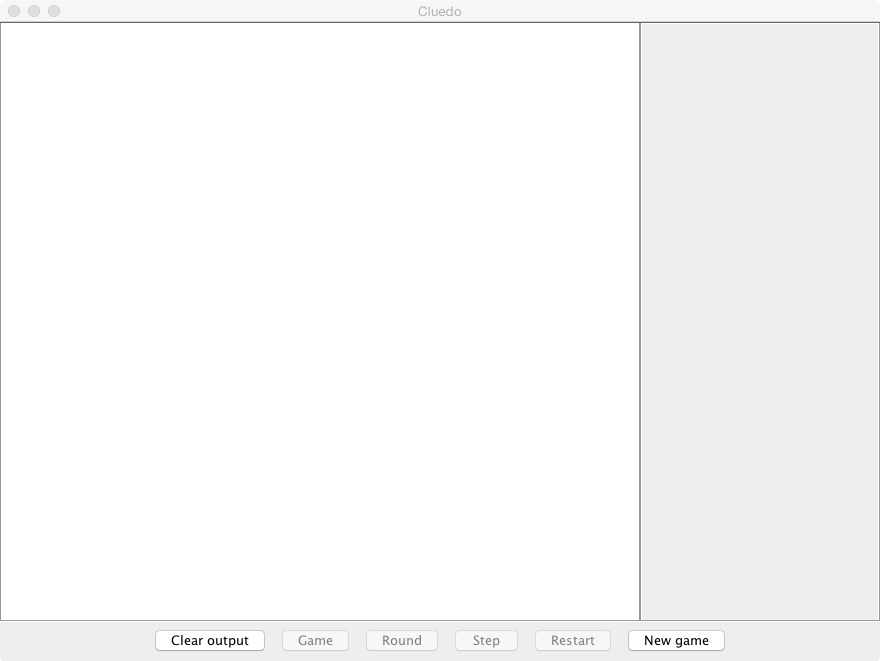
\includegraphics[height=0.8\textheight]{images/Empty}
\end{frame}

\begin{frame}{Runthrough}
    \centering
    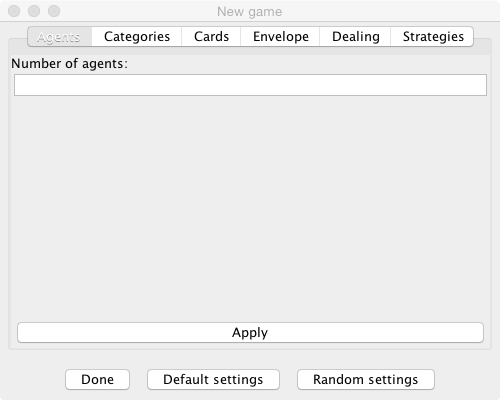
\includegraphics[height=0.8\textheight]{images/NewGame}
\end{frame}

\begin{frame}{Runthrough}
    \centering
    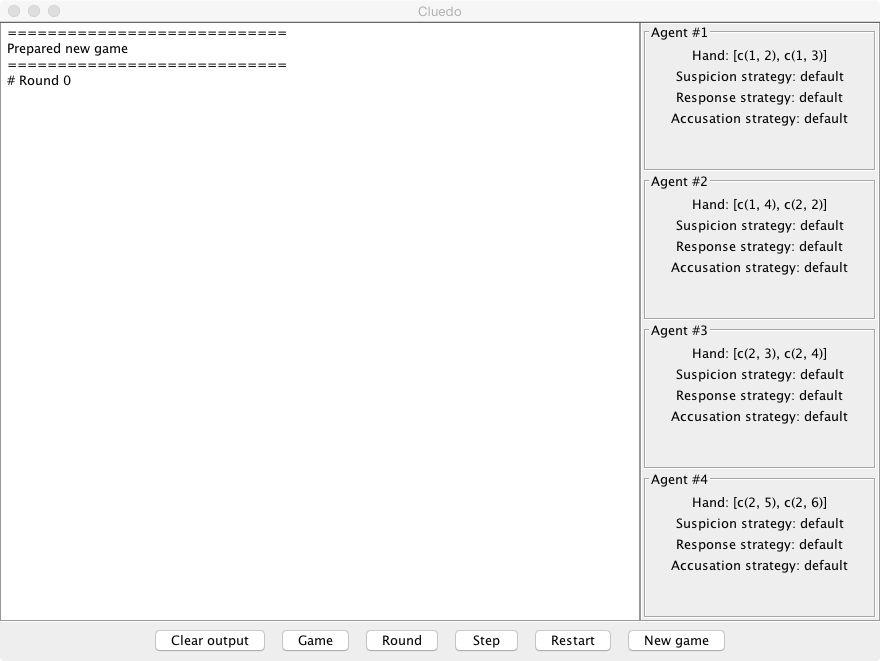
\includegraphics[height=0.8\textheight]{images/Prep}
\end{frame}

\begin{frame}{Runthrough}
    \centering
    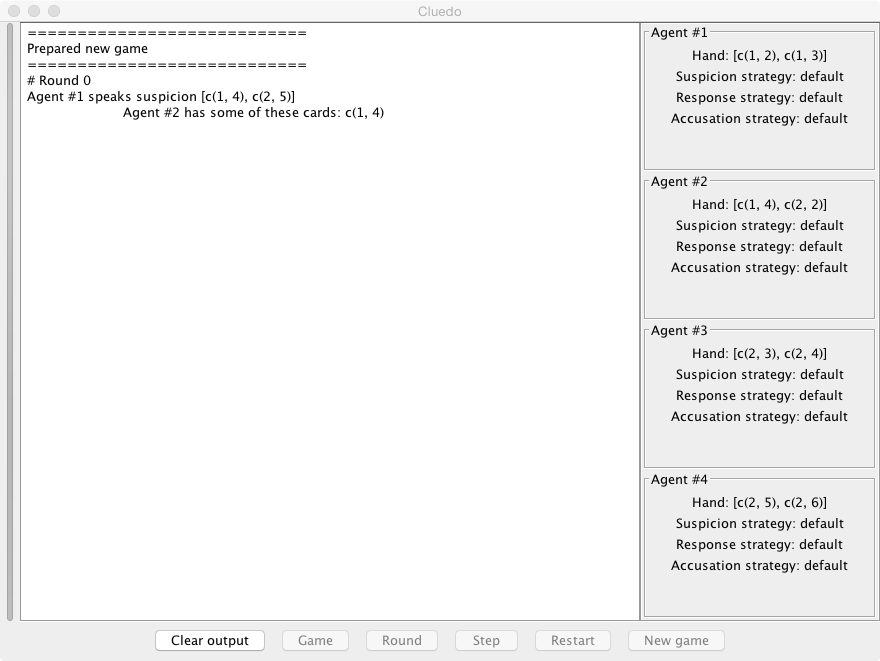
\includegraphics[height=0.8\textheight]{images/Running}
\end{frame}

\begin{frame}{Runthrough}
    \centering
    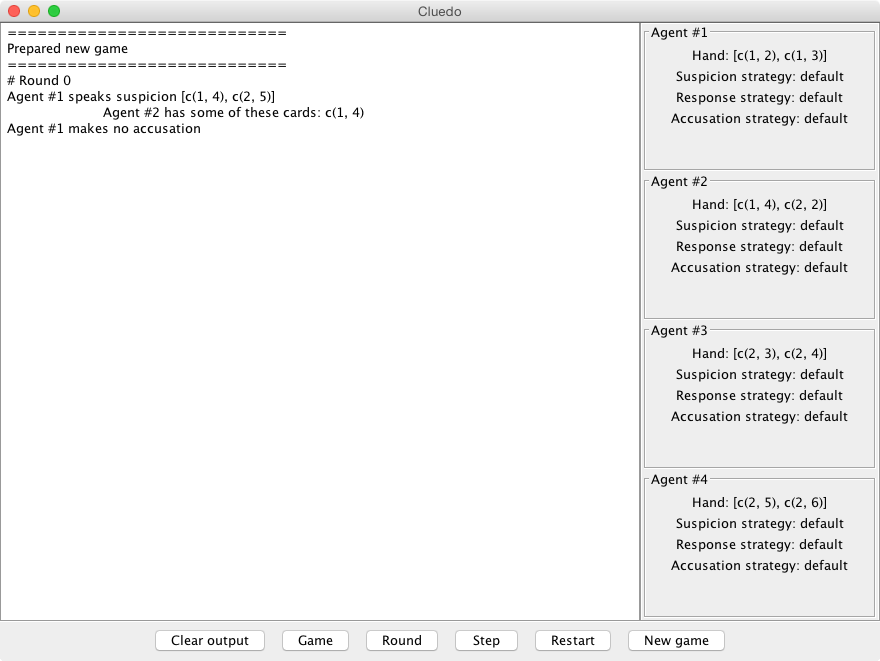
\includegraphics[height=0.8\textheight]{images/Stepped}
\end{frame}

\begin{frame}{Runthrough}
    \centering
    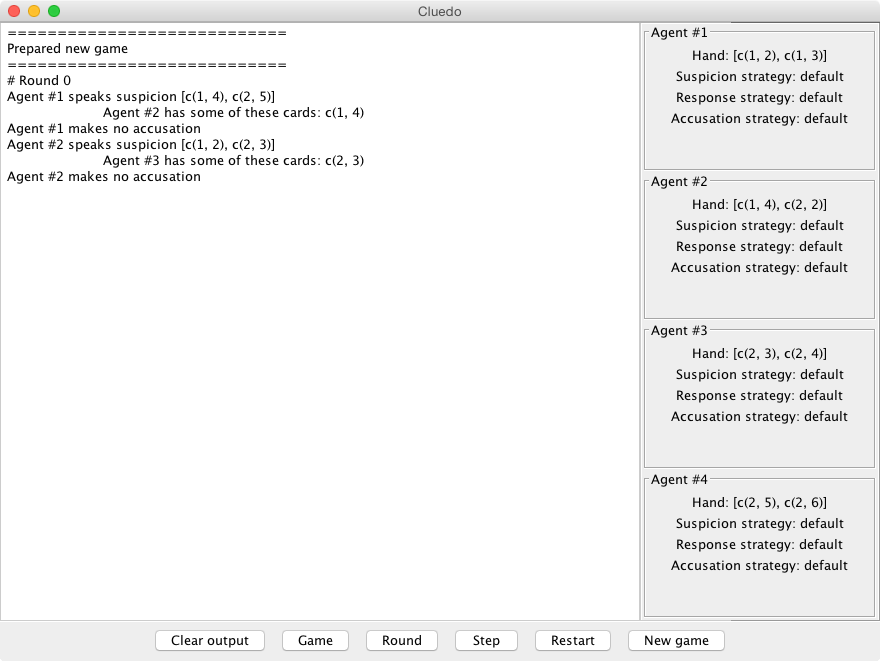
\includegraphics[height=0.8\textheight]{images/Step2}
\end{frame}

\begin{frame}{Runthrough}
    \centering
    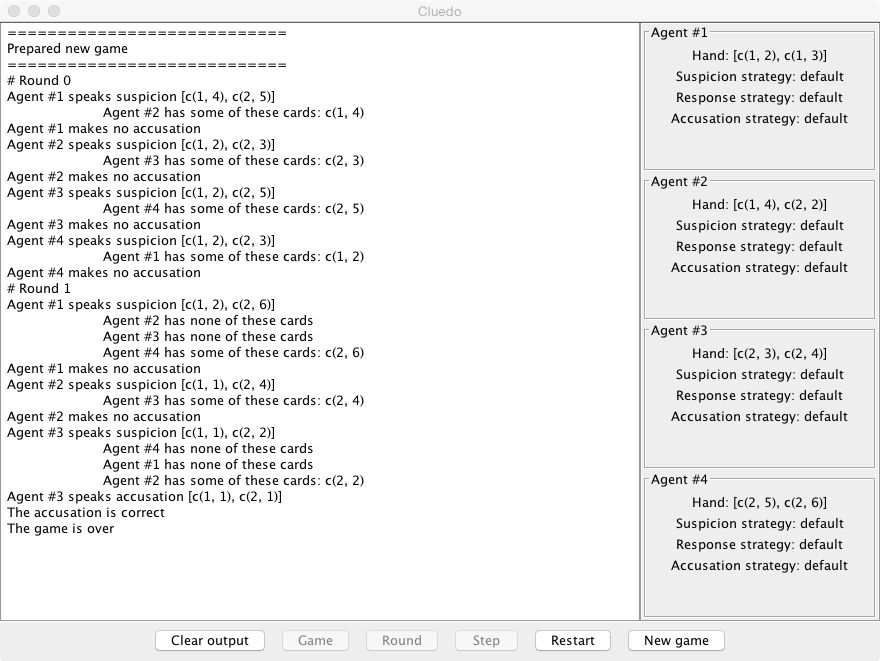
\includegraphics[height=0.8\textheight]{images/Done}
\end{frame}


\end{document}
